\textbf{\uline{Exemplo 20:}}
	\begin{center}
		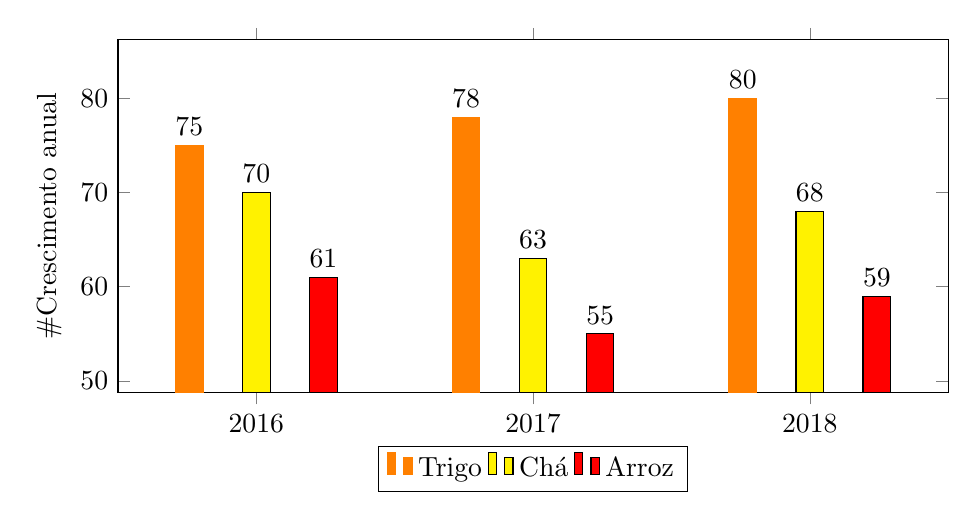
\begin{tikzpicture}  
			\begin{axis} 
				[ybar,enlargelimits=0.25,width=\textwidth, 
				height=0.5\textwidth,ybar=0.5cm,
				legend style={at={(0.5,-0.15)},    
					anchor=north,legend columns=3},     
				ylabel={\#Crescimento anual},
				symbolic x coords={2016, 2017, 2018},  
				xtick=data,  
				nodes near coords,  
				nodes near coords align={above}]  
				\addplot[fill=orange,draw=orange] coordinates {(2016, 75) (2017, 78) (2018, 80)};
				\addplot[fill=yellow] coordinates {(2016, 70) (2017, 63) (2018, 68)};  
				\addplot[fill=red] coordinates {(2016, 61) (2017, 55) (2018, 59)};  
				\legend{Trigo, Chá, Arroz}  
			\end{axis}  
		\end{tikzpicture}  
	\end{center}